\chapter{Migration strategy}
\label{chap:Chapter5}

This chapter defines a systematic strategy for migrating selected Boost libraries to Rust.
The strategy establishes a common methodology that is applicable to each of the selected libraries and provides
a structured approach for evaluating the resulting implementations.

The primary objective of the proposed strategy is to reproduce the relevant functionality of the selected Boost libraries in Rust 
while preserving their expected behavior and enabling their integration with existing C++ codebases. In addition, the strategy 
considers the requirements and constraints associated with the potential use of the migrated libraries in safety-critical 
automotive software architectures.

The migration strategy is divided into six main steps, described below:
\begin{enumerate}
\item \textbf{Understanding the library's functionality and its dependencies.}

The first step consists of analyzing the selected Boost library's source code, documentation and 
relevant technical literature, to understand its purpose, functionality, interfaces and dependencies.

This analysis identifies the relevant classes,funtions, data structures, algorithms, platform-specific
behavior and interactions with other libraries.
Particular attention is given to aspects that affect the observable behavior of the library and that may influence its migration to Rust.

A comprehensive understanding of these aspects is essential to ensure that the Rust implementation reproduces the relevant
semantics of the original library and can be subsequently be integrated into existing C++ codebases.

\item \textbf{Define Rust equivalents for the library's classes, functions, and data structures.}

Based on the analysus of the library's original implementation, the equivalent Rust abstractions
are defined for the library's classes, functions, data structures and interfaces. 

The Rust design does not necessarily replicate the structure of the original C++ implementation. 
Where appropriate, the design may differ in order to take advantage of Rust's ownership model,
type system, error handling mechanisms and idiomatic programmig practices, while preserving the required behavior of the original library.

\item \textbf{Implement the library's functionality in Rust, ensuring that it adheres to Rust's memory safety guarantees 
and best practices.}

The library's functionality is reimplemented in Rust. During this stage, particular attention is given to the Rust's ownership
and borrowing model, memory safety guarantees, error handling and idiomatic design principles. 

The implemenentation also considers the requirements and constraints of intended target environment.
Where the use of \texttt{unsafe} Rust is necessary, such usage should be minimized and restricted to well-defined boundaries, 
particularly when interacting with external code or platform-specific functionality.

\item \textbf{Create a C++ wrapper for the Rust implementation, allowing it to be used in existing C++ codebases.}

To enable integration with existing C++ codebases, an interoperability layer (C++ wrapper) is developed around the Rust implementation. 

The interoperability layer provides an interface suitable for use by the existing C++ applications while isolating the 
underlying Rust implementation from the consuming code.
Particular attention is given to the representation of data, ownership and object lifetime, error handling, memory management and 
the interaction between the C++ and Rust components.

\item \textbf{Test the Rust implementation and the C++ wrapper to ensure that they function correctly 
and meet performance requirements.}

The Rust implementation and its C++ wrapper are tested to verify functional correctness, behavioral equivalence with the original
Boost library where applicable, interoperability and performance. 

The original Boost implementation serves as a reference when behavioral compatibility is required. 
Equivalent inputs and relevant execution scenarios are used to identify discrepancies between the original and migrated implementations.

Performance evaluation is also performed to determine whether the Rust implementation and the 
interoperability layer introduce unacceptable overhead compared with the original implementation.

\item \textbf{Document the migration process, including any challenges encountered and solutions implemented, 
to provide guidance for future migrations of other Boost libraries to Rust.}

The final step consists of documenting the migration process, including design decisions, encoutered challenges, solutions, 
testing results and lessons learned. 

This documentation provides a reference for future migrations to other Boost libraries and 
contributes to the definition of a repeatable migration methodology.

\end{enumerate}

Among these steps, two are particularly critical for the success of the migration strategy. The first is the {analysis of 
the library's functionality and dependencies}, since an incomplete understanding of the original implementation can result in 
incorrect assumptions about its behavior or dependencies. The second is the \textbf{implementation of the functionality in Rust}, 
as this stage requires translating the original C++ abstractions into Rust while preserving the required semantics and taking 
advantage of Rust's memory safety guarantees and type system. These two stages therefore have a significant influence on the 
correctness and overall sucess of the migration.

\begin{figure}[H]
\centering
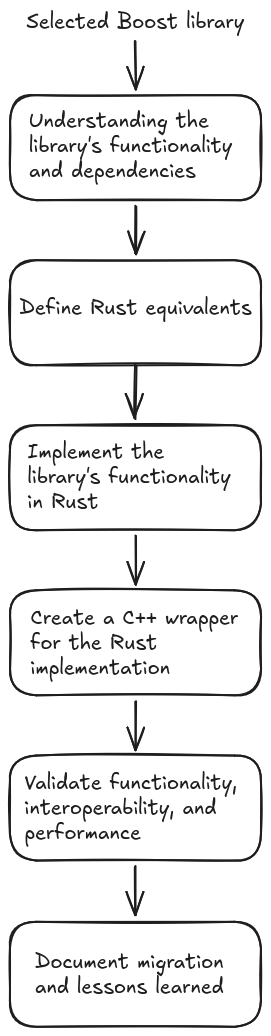
\includegraphics[width=0.25\textwidth]{ch5/assets/strategy.png}
\decoRule
\caption[Strategy]{Migration strategy}
\label{fig:Strategy}
\end{figure}

\newpage

The six steps described above can be grouped into four main phases, as follows:

\begin{enumerate}
\item \textbf{Analysis}
\begin{enumerate}
\item Understanding the library's functionality and dependencies.
\item Defining the migration scope and requirements.
\end{enumerate}
\item \textbf{Design and Implementation}
\begin{enumerate}
\item Defining the Rust equivalents of the relevant C++ abstractions.
\item Implementing the required functionality in Rust.
\end{enumerate}
\item \textbf{Interoperability}
\begin{enumerate}
\item Developing the interoperability layer between Rust and C++.
\end{enumerate}
\item \textbf{Validation and Evaluation}
\begin{enumerate}
\item Testing functional correctness, behavioral equivalence, interoperability, and performance.
\item Documenting the results, limitations, and lessons learned.
\end{enumerate}
\end{enumerate}

The phases are illustrated in Figure \ref{fig:Phases}.

\begin{figure}[H]
\centering
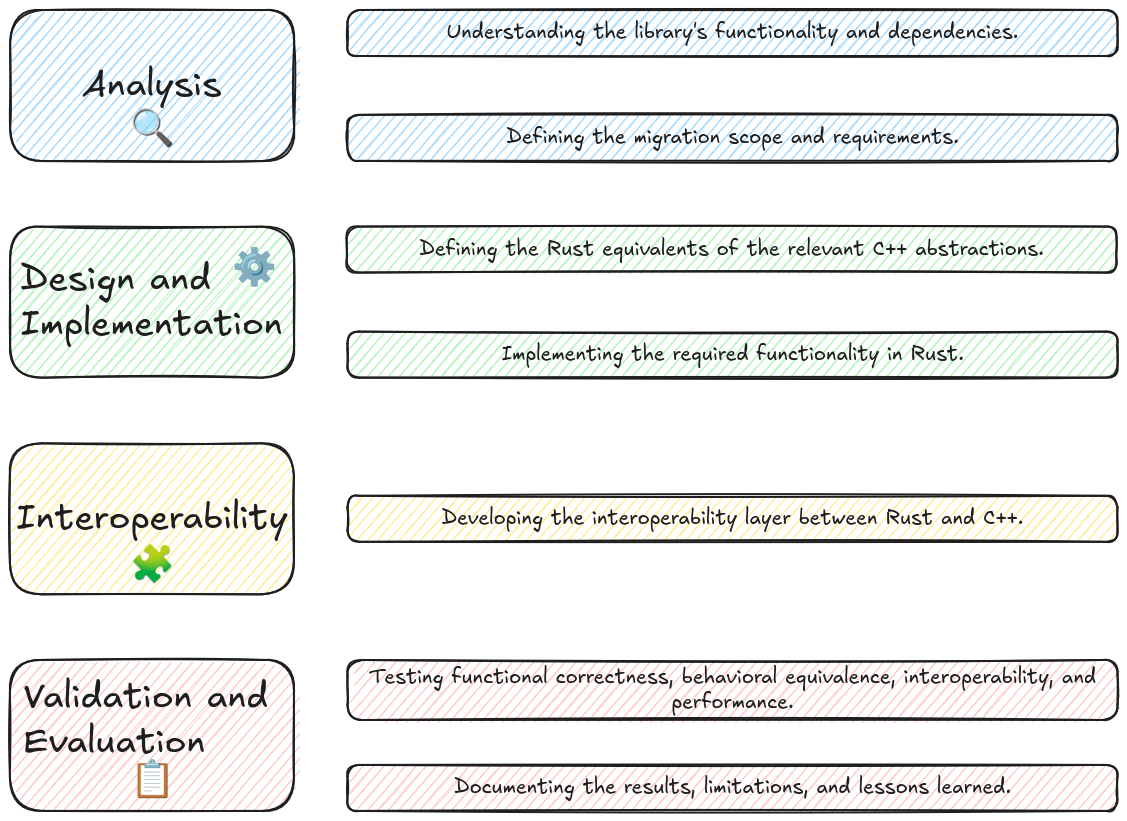
\includegraphics[width=0.8\textwidth]{ch5/assets/phases.png}
\decoRule
\caption{Migration phases}
\label{fig:Phases}
\end{figure}

\newpage

The migration strategy aims to satisfy the following objectives:

\begin{itemize}
\item Preserve the relevant behavior of the original Boost library;
\item Provide equivalent functionality through a Rust implementation;
\item Maintain interoperability with existing C++ applications;
\item Leverage Rust's memory and type safety guarantees;
\item Maintain acceptable performance compared with the original implementation;
\item Minimize and isolate the use of \texttt{unsafe} Rust, particularly at interoperability boundaries;
\item Consider the requirements and constraints of the intended automotive environment.
\end{itemize}

The success of a migration is therefore evaluated according to the extent to which these objectives are satisfied. 
The specific application of the proposed strategy, including the analysis, implementation, interoperability and 
evaluation of each selected Boost library, is presented in the following chapter.
